\PassOptionsToPackage{unicode=true}{hyperref} % options for packages loaded elsewhere
\PassOptionsToPackage{hyphens}{url}
\documentclass[11pt,dvipsnames,ignorenonframetext,aspectratio=169]{beamer}
\IfFileExists{pgfpages.sty}{\usepackage{pgfpages}}{}
\setbeamertemplate{caption}[numbered]
\setbeamertemplate{caption label separator}{: }
\setbeamercolor{caption name}{fg=normal text.fg}
\beamertemplatenavigationsymbolsempty
\usepackage{lmodern}
\usepackage{amssymb,amsmath}
\usepackage{ifxetex,ifluatex}
\usepackage{fixltx2e} % provides \textsubscript
\ifnum 0\ifxetex 1\fi\ifluatex 1\fi=0 % if pdftex
  \usepackage[T1]{fontenc}
  \usepackage[utf8]{inputenc}
\else % if luatex or xelatex
  \ifxetex
    \usepackage{mathspec}
  \else
    \usepackage{fontspec}
\fi
\defaultfontfeatures{Ligatures=TeX,Scale=MatchLowercase}







\fi

  \usetheme[]{monash}

  \usecolortheme{monashwhite}


% A default size of 24 is set in beamerthememonash.sty

% Title page
\setbeamertemplate{title page}
{\placefig{-0.01}{-0.01}{width=1.01\paperwidth,height=1.01\paperheight}{falcon.png}
% \begin{textblock}{7.5}(1,2.8)\usebeamerfont{title} % original
\begin{textblock}{15}(1,2.2)\usebeamerfont{title}
{\color{white}\raggedright\par\inserttitle}
\end{textblock}
\begin{textblock}{10}(1,6)
\small
{\color{white}\raggedright{\insertauthor}\mbox{}\\[0.1cm]
\insertdate}
\end{textblock}}


  \useinnertheme{rounded}

  \useoutertheme{smoothtree}

% use upquote if available, for straight quotes in verbatim environments
\IfFileExists{upquote.sty}{\usepackage{upquote}}{}
% use microtype if available
\IfFileExists{microtype.sty}{%
  \usepackage{microtype}
  \UseMicrotypeSet[protrusion]{basicmath} % disable protrusion for tt fonts
}{}


\newif\ifbibliography


\hypersetup{
      pdftitle={Quantitative genetics},
            colorlinks=true,
    linkcolor=red,
    citecolor=Blue,
    urlcolor=lightgrayd,
    breaklinks=true}
%\urlstyle{same}  % Use monospace font for urls







% Prevent slide breaks in the middle of a paragraph:
\widowpenalties 1 10000
\raggedbottom

  \AtBeginPart{
    \let\insertpartnumber\relax
    \let\partname\relax
    \frame{\partpage}
  }
  \AtBeginSection{
    \ifbibliography
    \else
      \let\insertsectionnumber\relax
      \let\sectionname\relax
      \frame{\sectionpage}
    \fi
  }
  \AtBeginSubsection{
    \let\insertsubsectionnumber\relax
    \let\subsectionname\relax
    \frame{\subsectionpage}
  }



\setlength{\parindent}{0pt}
\setlength{\parskip}{6pt plus 2pt minus 1pt}
\setlength{\emergencystretch}{3em}  % prevent overfull lines
\providecommand{\tightlist}{%
  \setlength{\itemsep}{0pt}\setlength{\parskip}{0pt}}

  \setcounter{secnumdepth}{0}


%% Monash overrides
\AtBeginSection[]{
   \frame<beamer>{
   \frametitle{Outline}\vspace*{0.2cm}
   
   \tableofcontents[currentsection,hideallsubsections]
  }}

% Redefine shaded environment if it exists (to ensure text is black)
\ifcsname Shaded\endcsname
  \definecolor{shadecolor}{RGB}{225,225,225}
  \renewenvironment{Shaded}{\color{black}\begin{snugshade}\color{black}}{\end{snugshade}}
\fi
%%

  \usepackage{setspace}
  \usepackage{wasysym}
  % \usepackage{footnote} % don't use this this breaks all
  \usepackage{fontenc}
  \usepackage{fontawesome}
  \usepackage{booktabs,siunitx}
  \usepackage{longtable}
  \usepackage{array}
  \usepackage{multirow}
  \usepackage{wrapfig}
  \usepackage{float}
  \usepackage{colortbl}
  \usepackage{pdflscape}
  \usepackage{tabu}
  \usepackage{threeparttable}
  \usepackage{threeparttablex}
  \usepackage[normalem]{ulem}
  \usepackage{makecell}
  \usepackage{xcolor}
  \usepackage{tikz} % required for image opacity change
  \usepackage[absolute,overlay]{textpos} % for text formatting
  \usepackage{chemfig}
  \usepackage[skip=0.333\baselineskip]{caption}
  % \newcommand*{\AlignChar}[1]{\makebox[1ex][c]{\ensuremath{\scriptstyle#1}}}%

  % this font option is amenable for beamer
  \setbeamerfont{caption}{size=\tiny}
  \singlespacing
  \definecolor{lightgrayd}{gray}{0.95}
  \definecolor{skyblued}{rgb}{0.65, 0.6, 0.94}
  \definecolor{oranged}{RGB}{245, 145, 200}

  \newlength{\cslhangindent}
  \setlength{\cslhangindent}{1.5em}
  \newenvironment{cslreferences}%
    {\setlength{\parindent}{0pt}%
    \everypar{\setlength{\hangindent}{\cslhangindent}}\ignorespaces}%
    {\par}

  \title[]{Quantitative genetics}


  \author[
        Deependra Dhakal\\
College of Natural Resource Management\\
Agriculture and Forestry University\\
\textit{ddhakal.rookie@gmail.com}\\
\url{https://rookie.rbind.io}
    ]{Deependra Dhakal\\
College of Natural Resource Management\\
Agriculture and Forestry University\\
\textit{ddhakal.rookie@gmail.com}\\
\url{https://rookie.rbind.io}}


\date[
      
  ]{
    }

\begin{document}

% Hide progress bar and footline on titlepage
  \begin{frame}[plain]
  \titlepage
  \end{frame}


   \frame<beamer>{
   \frametitle{Outline}\vspace*{0.2cm}
   
   \tableofcontents[hideallsubsections]
  }

\hypertarget{heterosis-and-inbreeding-depression}{%
\section{Heterosis and Inbreeding
depression}\label{heterosis-and-inbreeding-depression}}

\begin{frame}{Inbreeding depression}
\protect\hypertarget{inbreeding-depression}{}
\footnotesize

\begin{itemize}
\tightlist
\item
  Inbreeding depression is reduction in fitness as a direct result of
  inbreeding.
\item
  In theory, the heterosis observed on crossing is expected to be equal
  to the depression upon inbreeding, considering a large number of
  crosses between lines derived from a single base population.
\item
  In practice, plant breeders are interested in heterosis expressed by
  specific crosses between selected parents, or between populations that
  have no known common origin.
\item
  Reduction in fitness is usually manifested as a reduction in vigor,
  fertility, and productivity.
\item
  The effect is more severe in the early generations (5-8).
\item
  Plants including onions, sunflower, cucurbits, and rye are more
  tolerant of inbreeding with minimal consequences of inbreeding
  depression.
\item
  Plants such as alfalfa and carrot are highly intolerant of inbreeding.
\item
  A phenotypic measure of inbreeding depression is obtained through
  generational mean analysis. It is calculated as:
\end{itemize}

\[
\text{Inbreeding depression (ID)} = \frac{F_1 - F_2}{F_1} \times 100\%
\]
\end{frame}

\begin{frame}{}
\protect\hypertarget{section}{}
\begin{itemize}
\tightlist
\item
  Inbreeding is measured by the \textbf{Coefficient of Inbreeding}
  (\textbf{F}), which is the probability of identity of alleles by
  descent. The range of F is zero (no inbreeding; random mating) to one
  (prolonged selfing).
\item
  An unfit (deleterious) recessive allele is fairly quickly reduced in
  frequency but declines slowly thereafter.
\item
  On the other hand, an unfit dominant allele is rapidly eliminated from
  the population, while an intermediate allele is reduced more rapidly
  than a recessive allele because the former is open to selection in the
  heterozygote.
\item
  The consequence of these outcomes is that unfit dominant or
  intermediate alleles are rare in cross-breeding populations, while
  unfit recessive alleles persist because they are protected by their
  recessiveness.
\end{itemize}
\end{frame}

\begin{frame}{}
\protect\hypertarget{section-1}{}
\begin{columns}
\column{0.75\textwidth}
\begin{itemize}
\footnotesize
\item The alleles transmitted with each mating are labelled, $w, x, y~\text{and}~z$. We use "$\sim$" to symbolize IBD. We are interested to calculate the probability that $w$ and $x$ are IBD.
  \begin{itemize}
  \scriptsize
  \item The probability that "C" transmits the copy inherited from A to I, $P(x \sim y)$ = $\frac{1}{2}$
  \item The probability that "B" transmits the copy inherited from A to I, $P(w \sim z)$ = $\frac{1}{2}$
\end{itemize}
\item The probability that $z$ and $y$ are IBD can be through two ways:
  \begin{itemize}
  \scriptsize
  \item First way is when $z$ and $y$ are both the same copy (both pink or blue). This happens $\frac{1}{2}$ of the time since 1/4 of the time they are both blue and 1/4 both pink.
  \item Second way is when $z$ and $y$ are different copies (one pink and the other blue) but individual A was inbred. The probability that A's two copies are IBD is the inbreeding coefficient of A -- $F_A$. The probability that $z$ and $y$ are different copies that are IBD is $\frac{1}{2}\times F_A$.Thus,
  \end{itemize}
\end{itemize}

$$
\small
P(z \sim y) = \frac{1}{2} + \frac{1}{2}F_A
$$
\column{0.25\textwidth}

\begin{figure}
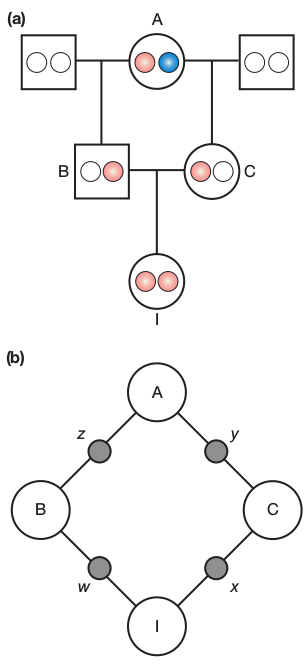
\includegraphics[width=0.65\linewidth]{../images/inbreeding_coefficient_half_sibs} \caption{\textbf{Inbreeding for half sibs.} B and C are half sibs who have the same mother, A, but different fathers; B and C have a daughter, I. Notice there is a closed loop from I through B and A and back to I through C. Since I's two copies of the gene trace back to the same copy in her grandmother, her two copies are identical by descent (IBD).}\label{fig:inbreeding-coefficient-in-half-sibs}
\end{figure}

\end{columns}
\end{frame}

\begin{frame}{}
\protect\hypertarget{section-2}{}
\begin{itemize}
\tightlist
\item
  Since, \(P(x \sim y), P(w \sim z),~\text{and},~P(z \sim y)\) are
  independent probabilities, product rule can be used to obtain combined
  probability.
\end{itemize}

\[
\begin{aligned}
F_I &= P(x \sim y)\times P(w \sim z) \times P(z \sim y) \\
&= \frac{1}{2} \times \frac{1}{2} \times \left( \frac{1}{2} + \frac{1}{2}F_A \right) \\
&= \left( \frac{1}{2} \right)^3 (1 + F_A)
\end{aligned}
\]

\begin{itemize}
\tightlist
\item
  If \(F_A\) for individual A is supposed to be 0, then
  \(F_I = \frac{1}{8}\).
\item
  \(\therefore\) Offspring of half-sib mating will be homozygous for
  alleles that are IBD for at least 1/8 (depending upon \(F_A\)) of
  their genes.
\end{itemize}
\end{frame}

\begin{frame}{}
\protect\hypertarget{section-3}{}
\begin{itemize}
\tightlist
\item
  In Figure \ref{fig:inbreeding-coefficient} (a) there is no inbreeding
  because there is no common ancestral pathway to the individual, A
  (i.e., all parents are different).
\item
  However, in Figure \ref{fig:inbreeding-coefficient} (b) inbreeding
  exists because B and C have common parents (D and E), that is, they
  are full sibs.
\item
  To calculate the amount of inbreeding, the standard pedigree is
  converted to an arrow diagram, as shown in
  \ref{fig:inbreeding-coefficient} (c).
\item
  Each individual contributes 1/2 of its genotype to its offspring. The
  \emph{coefficient of relationship} (R) is calculated by summing up all
  the pathways between two individuals through a common ancestor as:
  \(R_{BC} = \sum{\left(\frac{1}{2}\right)^s}\) , where s is the number
  of steps (arrows) from B to the common ancestor and back to C. For
  example, B and C probably inherited \((1/2)(1/2) = 1/4\) of their
  genes in common through ancestor D. Similarly, B and C probably
  inherited 1/4 of their genes in common through ancestor E.
\item
  The coefficient of relationship between B and C, as a result of common
  ancestry, is hence \(R_{BC} = 1/4 + 1/4 = 1/2 = 50\%\)
\end{itemize}
\end{frame}

\begin{frame}{}
\protect\hypertarget{section-4}{}
\begin{figure}

{\centering 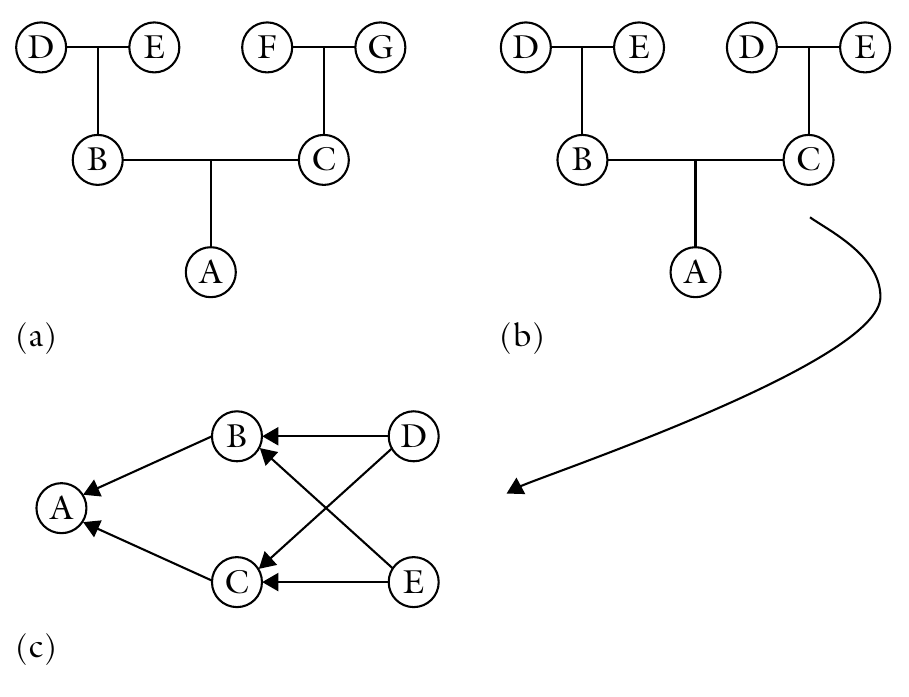
\includegraphics[width=0.45\linewidth]{../images/arrow_diagram} 

}

\caption{Pedigree diagrams can be drawn in the standard form (a, b) or converted to into an arrow diagram (c).}\label{fig:inbreeding-coefficient}
\end{figure}
\end{frame}

\begin{frame}{Heterosis (Hybrid vigor)}
\protect\hypertarget{heterosis-hybrid-vigor}{}
\begin{itemize}
\tightlist
\item
  Hybrid vigor may be defined as the increase in size, vigor, fertility,
  and overall productivity of a hybrid plant over the mid-parent value
  (average performance of the two parents).
\item
  It is calculated as the difference between the crossbred and inbred
  means:
\end{itemize}

\[\text{Hybrid vigour} = \frac{F_1-\frac{(P_1+P_2)}{2}}{\frac{(P_1+P_2)}{2}}\]

\begin{itemize}
\tightlist
\item
  The estimate is usually calculated as a percentage.
\item
  The synonymous term, heterosis, was coined by G.H. Shull.
\item
  Advantageous hybrid vigor is observed more frequently when breeders
  cross parents that are genetically diverse; When two inbred lines of
  outbred species are crossed.
\item
  The practical definition of heterosis is hybrid vigor that greatly
  exceeds the better or higher parent in a cross.
\item
  Hybrid breeding in maize quadrupled yields of maize in US between
  1930s and 1970s.
\end{itemize}
\end{frame}

\begin{frame}{Genetic basis of heterosis}
\protect\hypertarget{genetic-basis-of-heterosis}{}
\begin{itemize}
\tightlist
\item
  To explain the genetic basis for why fitness lost on inbreeding tends
  to be restored upon crossing, two theories have been proposed.

  \begin{itemize}
  \tightlist
  \item
    Dominance theory: C.G. Davenport in 1908 and later by I.M. Lerner,
  \item
    Overdominance theory: Shull in 1908 and later by K. Mather and J.L.
    Jinks.
  \end{itemize}
\item
  A third theory, the mechanism of epistasis (non-allelic gene
  interactions), has also been proposed.
\end{itemize}
\end{frame}

\begin{frame}{Dominance theory}
\protect\hypertarget{dominance-theory}{}
\footnotesize

\begin{itemize}
\tightlist
\item
  The dominance theory assumes that vigor in plants is conditioned by
  dominant alleles, recessive alleles being deleterious or neutral in
  effect.
\item
  It follows: a genotype with more dominant alleles will be more
  vigorous than one with few dominant alleles.
\item
  Consequently, crossing two parents with complementary dominant alleles
  will concentrate more favorable alleles in the hybrid than either
  parent.
\item
  In practice, if too many deleterious alleles are present, it makes it
  difficult to inbreed to recover sufficient loci with homozygous
  dominant alleles.
\item
  Inbreeding depression occurs upon selfing because the deleterious
  recessive alleles that are protected in the heterozygous condition
  (heterozygous advantage) become homozygous and are expressed.
\item
  Assume that each dominant genotype contributes 2 units to the
  phenotype, while a recessive genotype contributes 1 unit. A cross
  between two inbred parents could produce the following outcome:
\end{itemize}

\begin{center}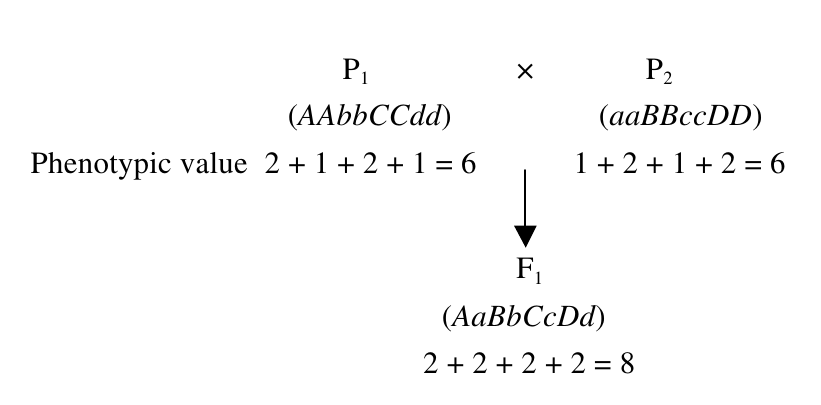
\includegraphics[width=0.35\linewidth]{../images/dominance_theory} \end{center}
\end{frame}

\begin{frame}{Overdominance theory}
\protect\hypertarget{overdominance-theory}{}
\footnotesize

\begin{itemize}
\tightlist
\item
  The phenomenon of the heterozygote being superior to the homozygote is
  called overdominance (i.e., heterozygosity \emph{per se} is assumed to
  be responsible for heterosis).
\item
  Theory assumes that the alleles of a gene (e.g., A, a) are contrasting
  but each has a different favorable effect in the plant.
\item
  A genotype with more heterozygous loci would be more vigorous than one
  with less heterozygotes.
\item
  Consider a quantitative trait conditioned by four loci, and assume
  that recessive, heterozygote, and homozygote dominants contribute 1,
  2, and 1.5 units to the phenotypic value, respectively:
\end{itemize}

\begin{center}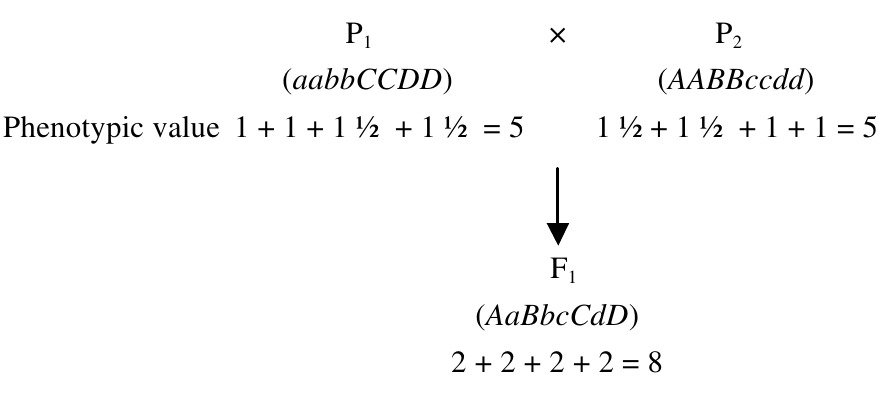
\includegraphics[width=0.3\linewidth]{../images/overdominance_theory} \end{center}
\end{frame}

\begin{frame}{Biometrics of heterosis}
\protect\hypertarget{biometrics-of-heterosis}{}
\begin{enumerate}
\tightlist
\item
  Better parent heterosis (Heterobeltiosis)
  \[Hybrid~vigour = \frac{F_1-Better~parent}{Better~parent}\]
\item
  Mid parent heterosis
  \[Hybrid~vigour = \frac{F_1-\frac{(P_1+P_2)}{2}}{\frac{(P_1+P_2)}{2}}\]
\item
  Commercial heterosis
  \[Hybrid~vigour = \frac{F_1-Commercial~Hybrid}{Commercial~Hybrid}\]
\end{enumerate}
\end{frame}

\begin{frame}{Types of hybrids}
\protect\hypertarget{types-of-hybrids}{}
\begin{itemize}
\tightlist
\item
  Commercial applications of hybrid breeding started with a cross of two
  inbred lines (a single cross - AxB) and later shifted to the more
  economic double cross, ({[}AxB{]}x{[}CxD{]}) and then back to a single
  cross.
\item
  Other parent combinations in hybrid development have been proposed,
  including the three-way cross ({[}AxB{]}xC) and modified versions of
  the single cross, in which closely related crosses showed that the
  single cross was superior in performance to the other two in terms of
  average yield.
\item
  However, it was noted also that the genotype x environment interaction
  (hybrid x environment) variability was more than twice that for the
  double crosses, while the mean variability for the three-way cross
  being intermediate.
\end{itemize}
\end{frame}

\begin{frame}{}
\protect\hypertarget{section-5}{}
\begin{itemize}
\tightlist
\item
  This indicated that the single crosses were more sensitive or
  responsive to environmental conditions than the other crosses.
\item
  Whereas high average yield is important to the producer, consistency
  in performance across years and locations (i.e., yield stability) is
  also important.
\item
  Double and three-way crosses have a more genetically divergent
  population for achieving buffering.
\item
  Today commercial hybrids are predominantly single cross, of best
  combining parental inbred lines.
\item
  For outline of mating scheme, See Lecture 7 on ``Hybridization
  techniques and its consequences'' (Course: Introductory plant
  breeding, \(4^{th}\) semester, BScAg).
\end{itemize}
\end{frame}

\begin{frame}{Numerical problem}
\protect\hypertarget{numerical-problem}{}
In blackgram, grain yield of parents (\(P_1\) and \(P_2\)) their \(F_1\)
and \(F_2\) progenies are given below:

\begin{table}
\centering\begingroup\fontsize{6}{8}\selectfont

\begin{tabular}{rrrr}
\toprule
Parent 1 & Parent 2 & F1 hybrid & F2 progeny\\
\midrule
19 & 23 & 29 & 15\\
\bottomrule
\end{tabular}
\endgroup{}
\end{table}

Calculate average heterosis, heterobeltiosis and inbreeding depression.
\end{frame}

\begin{frame}{Solution}
\protect\hypertarget{solution}{}
\begin{equation}
\begin{aligned}
\text{Mid parent heterosis} &= \frac{F_1 - MP}{MP} \times 100\% \\
\text{Here, Value of } F_1 &= 29.38 \\
\text{Mean of parents (MP)} &= \frac{18.9+22.69}{2} = 20.81 \\
\text{Mid parent heterosis } &= \frac{29.38-20.81}{20.81} \times 100\% = 41.12\% \\
\text{Heterobeltiosis} &= \frac{F_1-BP}{BP} \times 100\% = \frac{29.38-22.69}{22.69} \times 100\% = 29.48\% \\
\text{Inbreeding depression} &= \frac{F_1-F_2}{F_1} \times 100\% = \frac{29.38-15.18}{15.18} \times 100\%= 48.33\%
\end{aligned}
\nonumber
\end{equation}
\end{frame}

\hypertarget{inheritance-of-traits}{%
\section{Inheritance of traits}\label{inheritance-of-traits}}

\begin{frame}{Background}
\protect\hypertarget{background}{}
\begin{itemize}
\tightlist
\item
  The character may be simply inherited or complex inherited with effect
  of many genes at different loci, each contributing a small effect to
  phenotypic expression of the character

  \begin{enumerate}
  \tightlist
  \item
    Qualitative characters
  \item
    Quantitative characters
  \end{enumerate}
\item
  Study of inheritance of most characters/phenotypes can be classified
  into:

  \begin{enumerate}
  \tightlist
  \item
    Easily distinguished into discrete classes
  \end{enumerate}

  \begin{itemize}
  \tightlist
  \item
    barley plants may be

    \begin{itemize}
    \tightlist
    \item
      black or white hulled
    \item
      two or six rowed
    \item
      rough or smooth awned
    \item
      rust resistanct or rust susceptible
    \end{itemize}
  \end{itemize}
\end{itemize}
\end{frame}

\begin{frame}{}
\protect\hypertarget{section-6}{}
\begin{enumerate}
\setcounter{enumi}{1}
\tightlist
\item
  Cannot be easily classified into discrete classes - for grain yield
  \(kg~ha^{-1}\)

  \begin{itemize}
  \tightlist
  \item
    thousand grain weight (gram),
  \item
    plant height (cm) variation may be differing by small units
  \end{itemize}
\end{enumerate}
\end{frame}

\begin{frame}{Quantitative inheritance}
\protect\hypertarget{quantitative-inheritance}{}
\begin{itemize}
\tightlist
\item
  Most of the important variation displayed by nearly all plant traits
  affecting growth, development and reproduction, is quantitative.
\item
  Also called: \emph{Continuous}, \emph{Polygenic variation},
  \emph{Multiple gene controlled traits}
\item
  Demonstrate same basic Mendelian properties for a gene, and also the
  Hardy-Weinberg equilibrium.
\item
  Quantitative characters are governed by several genes; each gene has a
  small effect, which is usually cumulative.
\item
  The environments considerably affect these characters.
\item
  Quantitative characters often show continuous variation with normal
  distribution
\end{itemize}
\end{frame}

\begin{frame}{Qualitative inheritance}
\protect\hypertarget{qualitative-inheritance}{}
\begin{itemize}
\tightlist
\item
  Mendel purposed the law of inheritance based on his studies with
  qualitative characters.
\item
  In the studies of qualitative inheritance, we study phenomena such as:

  \begin{enumerate}
  \tightlist
  \item
    Dominance,
  \item
    Segregation and independent assortment,
  \item
    Gene action and interactions (Epistatis, Masking gene action,
    Duplicate gene action, Complementary gene action, Additive gene
    action, Inhibiting gene action, Modifying gene action and
    Pleiotropy).
  \item
    Penetrance and expressivity
  \item
    Linkage
  \end{enumerate}
\end{itemize}
\end{frame}

\begin{frame}{Difference}
\protect\hypertarget{difference}{}
\begin{table}

\caption{\label{tab:quality-quantity-difference}Difference between qualitative and quantitative traits}
\centering
\fontsize{6}{8}\selectfont
\begin{tabular}[t]{>{\raggedright\arraybackslash}p{12em}>{\raggedright\arraybackslash}p{12em}>{\raggedright\arraybackslash}p{12em}}
\toprule
Character & Qualitative & Quantitative\\
\midrule
Number of gene and loci controlling the character & Few, one (mongenic) or few major genes (oligogenic) & Many, polygenes (polygeneic)\\
Effect of individual gene & Large & Small\\
Follow mendel's law & Yes & Yes\\
Classification on few discrete classes that are easily distinguished & Yes & No\\
Measurement of the character & Observation & Measured in metric units\\
\addlinespace
Frequency distribution & Discrete & Continuous and often normal\\
Effect of environment on expression of character & No or little affected & Largely affected\\
Examples & Disease resistance, Presence of awns, Seed color & Grain yield (kg/ha), Thousand kernel weight (gram)\\
\bottomrule
\end{tabular}
\end{table}
\end{frame}

\hypertarget{johanssens-pureline-theory}{%
\section{Johanssen's pureline theory}\label{johanssens-pureline-theory}}

\begin{frame}{Pureline theory}
\protect\hypertarget{pureline-theory}{}
\begin{itemize}
\tightlist
\item
  Johannsen demonstrated that a mixed population of self-pollinated
  species could be sorted out into genetically pure lines.
\item
  These lines were subsequently non-responsive to selection within each
  of them.
\item
  Lines that are genetically different may be successfully isolated from
  within a population of mixed genetic types.
\item
  Any variation that occurs within a pure line is not heritable but due
  to environmental factors only. Consequently, as Johansen's bean study
  showed, further selection within the line is not effective.
\end{itemize}
\end{frame}

\begin{frame}{}
\protect\hypertarget{section-7}{}
\begin{figure}

{\centering 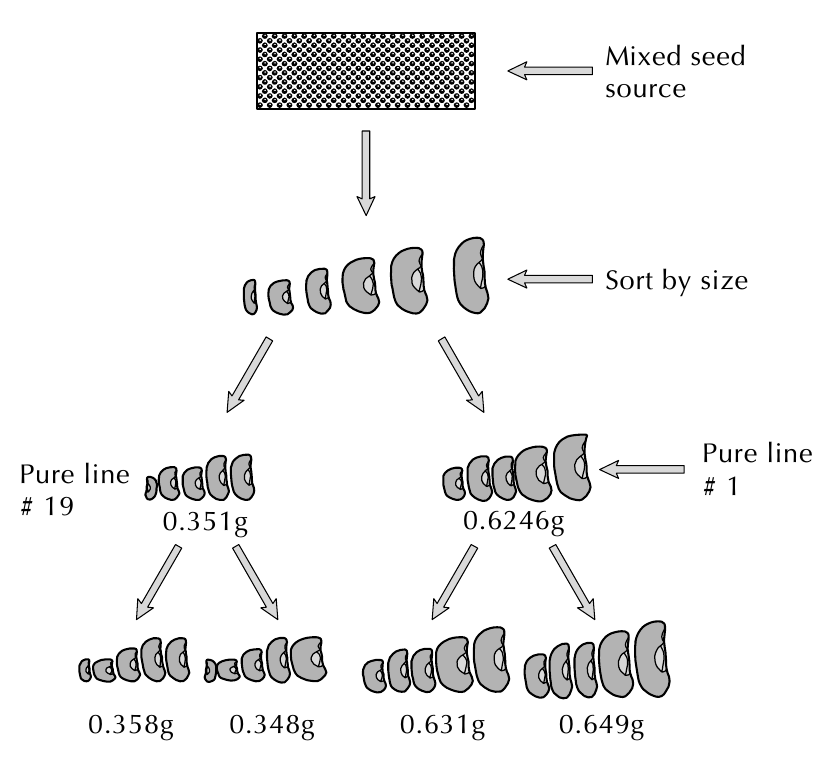
\includegraphics[width=0.45\linewidth]{../images/johannsens_purlines} 

}

\caption{Johannsen's observation of Phaseolus bean shed light on Pureline theory}\label{fig:johannsens-purelines}
\end{figure}
\end{frame}

\begin{frame}{}
\protect\hypertarget{section-8}{}
\begin{itemize}
\tightlist
\item
  Lines are used

  \begin{itemize}
  \tightlist
  \item
    as cultivars or as parents in hybrid production (inbred lines).
  \item
    in the development of genetic stock (containing specific genes such
    as disease resistance, nutritional quality) and synthetic and
    multiline cultivars.
  \end{itemize}
\item
  Line cultivars have a very narrow genetic base and tend to be uniform
  in traits of interest (e.g., height, maturity).
\end{itemize}
\end{frame}

\begin{frame}{Application}
\protect\hypertarget{application}{}
\begin{itemize}
\tightlist
\item
  Cultivars for mechanized production that must meet a certain
  specification for uniform operation by farm machines (e.g., uniform
  maturity, uniform height for uniform location of economic part).
\item
  Cultivars developed for a discriminating market that puts a premium on
  eye-appeal (e.g., uniform shape, size).
\item
  Cultivars for the processing market (e.g., with demand for certain
  canning qualities, texture).
\item
  Advancing ``sports'' that appear in a population (e.g., a mutant
  flower for ornamental use).
\item
  Improving newly domesticated crops that have some variability.
\item
  The pure-line selection method is also an integral part of other
  breeding method,s such as the pedigree selection and bulk population
  selection.
\end{itemize}
\end{frame}

\begin{frame}{Overview}
\protect\hypertarget{overview}{}
\begin{itemize}
\tightlist
\item
  The pure-line selection in breeding entails repeated cycles of selfing
  following the initial selection from a mixture of homozygous lines.
\item
  Natural populations of self-pollinated species consist of mixtures of
  homozygous lines with transient heterozygosity originating from
  mutations and outcrossing.
\item
  Steps:

  \begin{itemize}
  \tightlist
  \item
    Year 1: The first step is to obtain a variable base population
    (e.g., introductions, segregating populations from crosses, land
    race) and space plant it in the first year, select, and harvest
    desirable individuals.
  \item
    Year 2: Grow progeny rows of selected plants. Rogue out any
    variants. Harvest selected progenies individually. These are
    experimental strains.
  \item
    Year 3-6: Conduct preliminary yield trials of the experimental
    strains including appropriate check cultivars.
  \item
    Year 7-10: Conduct advanced yield trials at multilocations. Release
    highest yielding line as new cultivar.
  \end{itemize}
\end{itemize}
\end{frame}

\begin{frame}{}
\protect\hypertarget{section-9}{}
\begin{figure}

{\centering 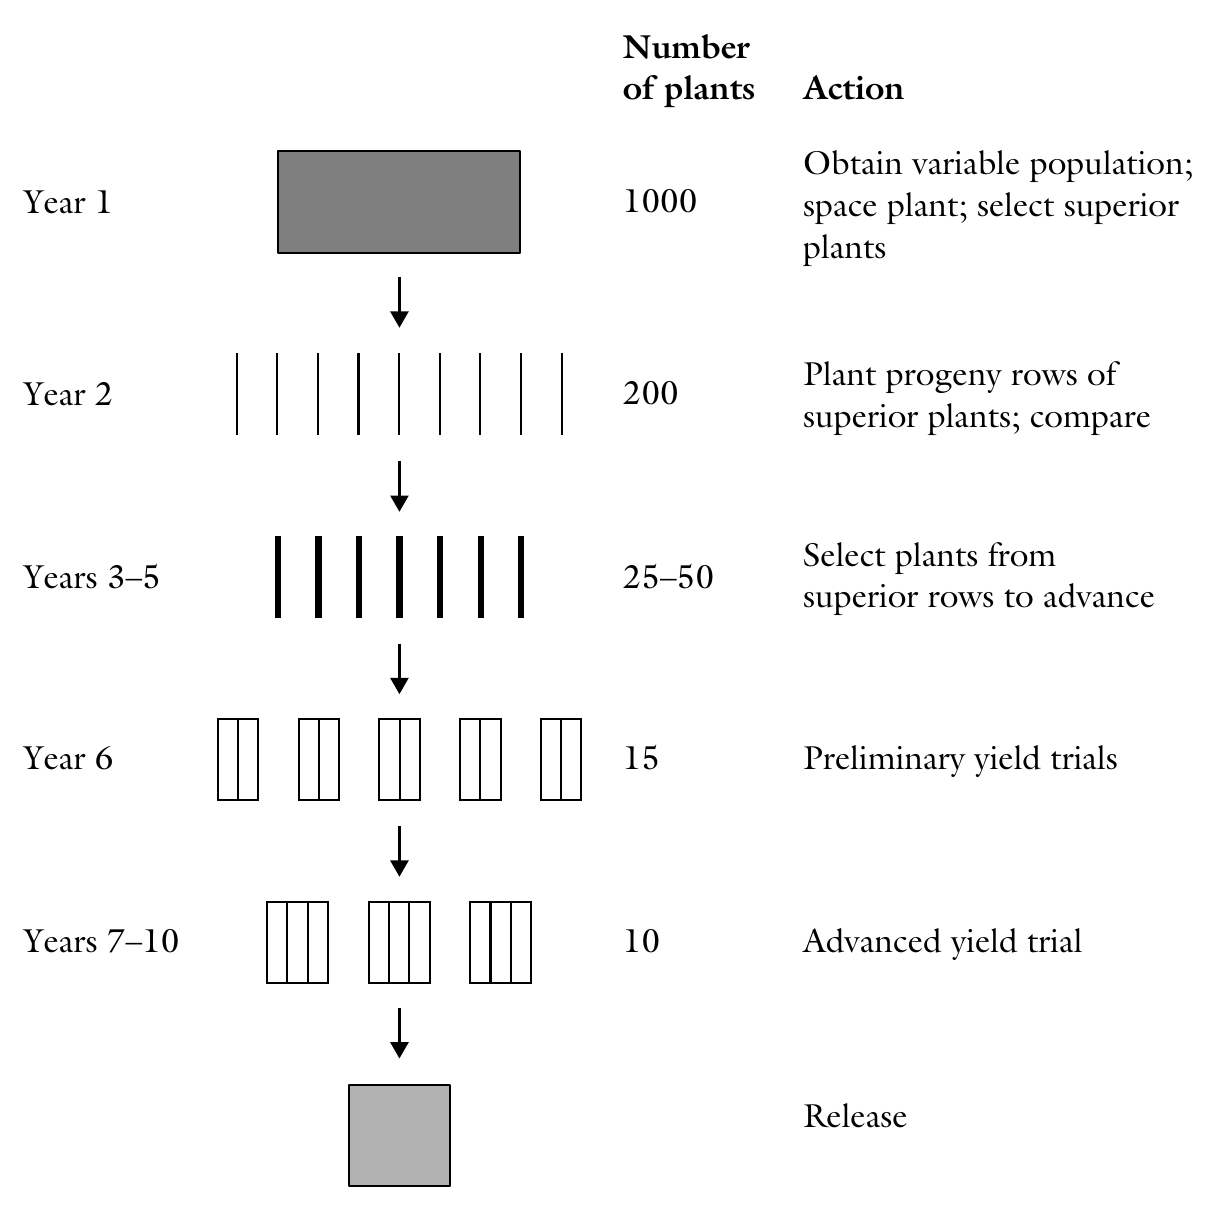
\includegraphics[width=0.45\linewidth]{../images/pureline_selection} 

}

\caption{Generalized steps in breeding by pure-line selection}\label{fig:pureline-selection}
\end{figure}
\end{frame}

\begin{frame}{Genetic issues}
\protect\hypertarget{genetic-issues}{}
\begin{itemize}
\tightlist
\item
  Pure-line breeding produces cultivars with a narrow genetic base and,
  hence, that are less likely to produce stable yields over a wider
  range of environments. Such cultivars are more prone to being wiped
  out by pathogenic outbreaks.
\item
  Pure-line cultivars depend primarily on phenotypic plasticity for
  production response and stability across environments.
\end{itemize}
\end{frame}

\begin{frame}{Advantages}
\protect\hypertarget{advantages}{}
\begin{itemize}
\tightlist
\item
  It is a rapid breeding method.
\item
  The method is inexpensive to conduct. The base population can be a
  landrace. The population size selected is variable and can be small or
  large, depending on the objective.
\item
  The cultivar developed by this method has great ``eye appeal''
  (because of the high uniformity of, e.g., harvesting time, height,
  etc.).
\end{itemize}
\end{frame}

\begin{frame}{Disadvantages}
\protect\hypertarget{disadvantages}{}
\begin{itemize}
\tightlist
\item
  The purity of the cultivar may be altered through admixture, natural
  crossing with other cultivars, and mutations. Such off-type plants
  should be rogued out to maintain cultivar purity.
\item
  The cultivar has a narrow genetic base and, hence, is susceptible to
  devastation from adverse environmental factors because of uniform
  response.
\item
  A new genotype is not created. Rather, improvement is limited to the
  isolation of the most desirable or best genotype from a mixed
  population.
\item
  The method promotes genetic erosion because most superior pure lines
  are identified and multiplied to the exclusion of other genetic
  variants.
\item
  Progeny rows takes up more resources (time, space, funds).
\end{itemize}
\end{frame}

\hypertarget{polygenes-in-discontinuous-traits}{%
\section{Polygenes in discontinuous
traits}\label{polygenes-in-discontinuous-traits}}

\begin{frame}{}
\protect\hypertarget{section-10}{}
\begin{itemize}
\tightlist
\item
  Polygenes are genes with effects that are too small to be individually
  distinguished. They are sometimes called \textbf{minor genes}
\item
  Most of the important variation displayed by nearly all plant traits
  affecting growth, development and reproduction, is quantitative
  (continuous or polygenic variation; controlled by many genes).
\item
  Polygenes demonstrate the same properties in terms of dominance,
  epistasis, and linkage as classical Mendelian genes.
\end{itemize}
\end{frame}

\begin{frame}{}
\protect\hypertarget{section-11}{}
\begin{itemize}
\tightlist
\item
  In many cases discontinuous or stepwise distinction between phenotypes
  inevitably accompany measurements for a praticular characteristic.
\item
  For example, the number of vertebrae in some species of chordates may
  differ between individuals, but the difference is generally classified
  on the basis of whole numbers of vertebrae, or, as in resistance to
  disease, the character is expressed in an ``all or none'' fashion.
\item
  Such characters may nevertheless be influenced by numerous polygenes.
\end{itemize}
\end{frame}

\begin{frame}{}
\protect\hypertarget{section-12}{}
\begin{itemize}
\tightlist
\item
  Polygenes and their expression of discontinuous characters comes about
  through the establishment of ``thresholds.'' Expression of particular
  phenotypes of polygenic genotypes occur only when the genotypes have
  values above this threshold.
\item
  Thus, although there is superficial discontinuous phenotypic
  distribution, there underlies a continuous polygenic distribution.
\item
  Wright first demonstrated the \textbf{relationship between two scales}
  in crosses between strains of guinea pigs, that differed from each
  other in the \textbf{number of toes on the hind leg}.
\end{itemize}
\end{frame}

\begin{frame}{}
\protect\hypertarget{section-13}{}
\begin{itemize}
\tightlist
\item
  One strain (number 2) had the normal three toes on hind leg, and the
  other (D) was polydactylous, with four toes.
\item
  Their \(F_1\) offspring were 3 toed, as expected.
\item
  In \(F_2\), however, ratio of
  \(\text{Three toed: Four toed } \simeq 3:1\) (188:45 individuals).
\item
  It seems as if these crosses were segregating for only a single gene
  difference in the \(F_2\). This was further corroborated by the
  testcross results.
\item
  In the testcross however, one gene hypothesis was evidently disproved
  with the observation that three-toed parental type was not
  heterozygous.
\item
  On the contrary, wright found that backcrossing these three-toed
  ``heterozygotes'' to the four-toed stock resulted in 77 percent
  four-toed to 23 percent three-toed offspring.
\end{itemize}
\end{frame}

\begin{frame}{}
\protect\hypertarget{section-14}{}
\begin{itemize}
\tightlist
\item
  With support of other evidence, wright proposed that polydactyly is
  affected by four pair of polygens (8 alleles).
\item
  Individuals which had about five or more polydactylous alleles out of
  eight had exceeded the ``threshold'' and appeared as four toed.
\item
  Initial four toed stock was therefore entirely of this type.
\item
  Since parental three-toed stock had its polygenic distribution
  centered far below the threshold, \(F_1\) hybrids were mostly three
  toed.
\end{itemize}
\end{frame}

\begin{frame}{}
\protect\hypertarget{section-15}{}
\renewcommand{\arraystretch}{2}

\begin{table}
\centering\begingroup\fontsize{6}{8}\selectfont

\resizebox{\linewidth}{!}{
\begin{tabular}{lllllllllllllllll}
\toprule
Gamete types & abcd & abcD & abCd & abCD & aBcd & aBcD & aBCd & aBCD & Abcd & AbcD & AbCd & AbCD & ABcd & ABcD & ABCd & ABCD\\
\midrule
abcd & \cellcolor[HTML]{a8a035}{aabbccdd} & \cellcolor[HTML]{a8a035}{aabbccdD} & \cellcolor[HTML]{a8a035}{aabbcCdd} & \cellcolor[HTML]{a8a035}{aabbcCdD} & \cellcolor[HTML]{a8a035}{aabBccdd} & \cellcolor[HTML]{a8a035}{aabBccdD} & \cellcolor[HTML]{a8a035}{aabBcCdd} & \cellcolor[HTML]{a8a035}{aabBcCdD} & \cellcolor[HTML]{a8a035}{aAbbccdd} & \cellcolor[HTML]{a8a035}{aAbbccdD} & \cellcolor[HTML]{a8a035}{aAbbcCdd} & \cellcolor[HTML]{a8a035}{aAbbcCdD} & \cellcolor[HTML]{a8a035}{aAbBccdd} & \cellcolor[HTML]{a8a035}{aAbBccdD} & \cellcolor[HTML]{a8a035}{aAbBcCdd} & \cellcolor[HTML]{802acc}{aAbBcCdD}\\
abcD & \cellcolor[HTML]{a8a035}{aabbccdD} & \cellcolor[HTML]{a8a035}{aabbccDD} & \cellcolor[HTML]{a8a035}{aabbcCdD} & \cellcolor[HTML]{a8a035}{aabbcCDD} & \cellcolor[HTML]{a8a035}{aabBccdD} & \cellcolor[HTML]{a8a035}{aabBccDD} & \cellcolor[HTML]{a8a035}{aabBcCdD} & \cellcolor[HTML]{802acc}{aabBcCDD} & \cellcolor[HTML]{a8a035}{aAbbccdD} & \cellcolor[HTML]{a8a035}{aAbbccDD} & \cellcolor[HTML]{a8a035}{aAbbcCdD} & \cellcolor[HTML]{802acc}{aAbbcCDD} & \cellcolor[HTML]{a8a035}{aAbBccdD} & \cellcolor[HTML]{802acc}{aAbBccDD} & \cellcolor[HTML]{802acc}{aAbBcCdD} & \cellcolor[HTML]{802acc}{aAbBcCDD}\\
abCd & \cellcolor[HTML]{a8a035}{aabbcCdd} & \cellcolor[HTML]{a8a035}{aabbcCdD} & \cellcolor[HTML]{a8a035}{aabbCCdd} & \cellcolor[HTML]{a8a035}{aabbCCdD} & \cellcolor[HTML]{a8a035}{aabBcCdd} & \cellcolor[HTML]{a8a035}{aabBcCdD} & \cellcolor[HTML]{a8a035}{aabBCCdd} & \cellcolor[HTML]{802acc}{aabBCCdD} & \cellcolor[HTML]{a8a035}{aAbbcCdd} & \cellcolor[HTML]{a8a035}{aAbbcCdD} & \cellcolor[HTML]{a8a035}{aAbbCCdd} & \cellcolor[HTML]{802acc}{aAbbCCdD} & \cellcolor[HTML]{a8a035}{aAbBcCdd} & \cellcolor[HTML]{802acc}{aAbBcCdD} & \cellcolor[HTML]{802acc}{aAbBCCdd} & \cellcolor[HTML]{802acc}{aAbBCCdD}\\
abCD & \cellcolor[HTML]{a8a035}{aabbcCdD} & \cellcolor[HTML]{a8a035}{aabbcCDD} & \cellcolor[HTML]{a8a035}{aabbCCdD} & \cellcolor[HTML]{802acc}{aabbCCDD} & \cellcolor[HTML]{a8a035}{aabBcCdD} & \cellcolor[HTML]{802acc}{aabBcCDD} & \cellcolor[HTML]{802acc}{aabBCCdD} & \cellcolor[HTML]{802acc}{aabBCCDD} & \cellcolor[HTML]{a8a035}{aAbbcCdD} & \cellcolor[HTML]{802acc}{aAbbcCDD} & \cellcolor[HTML]{802acc}{aAbbCCdD} & \cellcolor[HTML]{802acc}{aAbbCCDD} & \cellcolor[HTML]{802acc}{aAbBcCdD} & \cellcolor[HTML]{802acc}{aAbBcCDD} & \cellcolor[HTML]{802acc}{aAbBCCdD} & \cellcolor[HTML]{802acc}{aAbBCCDD}\\
aBcd & \cellcolor[HTML]{a8a035}{aabBccdd} & \cellcolor[HTML]{a8a035}{aabBccdD} & \cellcolor[HTML]{a8a035}{aabBcCdd} & \cellcolor[HTML]{a8a035}{aabBcCdD} & \cellcolor[HTML]{a8a035}{aaBBccdd} & \cellcolor[HTML]{a8a035}{aaBBccdD} & \cellcolor[HTML]{a8a035}{aaBBcCdd} & \cellcolor[HTML]{802acc}{aaBBcCdD} & \cellcolor[HTML]{a8a035}{aAbBccdd} & \cellcolor[HTML]{a8a035}{aAbBccdD} & \cellcolor[HTML]{a8a035}{aAbBcCdd} & \cellcolor[HTML]{802acc}{aAbBcCdD} & \cellcolor[HTML]{a8a035}{aABBccdd} & \cellcolor[HTML]{802acc}{aABBccdD} & \cellcolor[HTML]{802acc}{aABBcCdd} & \cellcolor[HTML]{802acc}{aABBcCdD}\\
aBcD & \cellcolor[HTML]{a8a035}{aabBccdD} & \cellcolor[HTML]{a8a035}{aabBccDD} & \cellcolor[HTML]{a8a035}{aabBcCdD} & \cellcolor[HTML]{802acc}{aabBcCDD} & \cellcolor[HTML]{a8a035}{aaBBccdD} & \cellcolor[HTML]{802acc}{aaBBccDD} & \cellcolor[HTML]{802acc}{aaBBcCdD} & \cellcolor[HTML]{802acc}{aaBBcCDD} & \cellcolor[HTML]{a8a035}{aAbBccdD} & \cellcolor[HTML]{802acc}{aAbBccDD} & \cellcolor[HTML]{802acc}{aAbBcCdD} & \cellcolor[HTML]{802acc}{aAbBcCDD} & \cellcolor[HTML]{802acc}{aABBccdD} & \cellcolor[HTML]{802acc}{aABBccDD} & \cellcolor[HTML]{802acc}{aABBcCdD} & \cellcolor[HTML]{802acc}{aABBcCDD}\\
aBCd & \cellcolor[HTML]{a8a035}{aabBcCdd} & \cellcolor[HTML]{a8a035}{aabBcCdD} & \cellcolor[HTML]{a8a035}{aabBCCdd} & \cellcolor[HTML]{802acc}{aabBCCdD} & \cellcolor[HTML]{a8a035}{aaBBcCdd} & \cellcolor[HTML]{802acc}{aaBBcCdD} & \cellcolor[HTML]{802acc}{aaBBCCdd} & \cellcolor[HTML]{802acc}{aaBBCCdD} & \cellcolor[HTML]{a8a035}{aAbBcCdd} & \cellcolor[HTML]{802acc}{aAbBcCdD} & \cellcolor[HTML]{802acc}{aAbBCCdd} & \cellcolor[HTML]{802acc}{aAbBCCdD} & \cellcolor[HTML]{802acc}{aABBcCdd} & \cellcolor[HTML]{802acc}{aABBcCdD} & \cellcolor[HTML]{802acc}{aABBCCdd} & \cellcolor[HTML]{802acc}{aABBCCdD}\\
aBCD & \cellcolor[HTML]{a8a035}{aabBcCdD} & \cellcolor[HTML]{802acc}{aabBcCDD} & \cellcolor[HTML]{802acc}{aabBCCdD} & \cellcolor[HTML]{802acc}{aabBCCDD} & \cellcolor[HTML]{802acc}{aaBBcCdD} & \cellcolor[HTML]{802acc}{aaBBcCDD} & \cellcolor[HTML]{802acc}{aaBBCCdD} & \cellcolor[HTML]{802acc}{aaBBCCDD} & \cellcolor[HTML]{802acc}{aAbBcCdD} & \cellcolor[HTML]{802acc}{aAbBcCDD} & \cellcolor[HTML]{802acc}{aAbBCCdD} & \cellcolor[HTML]{802acc}{aAbBCCDD} & \cellcolor[HTML]{802acc}{aABBcCdD} & \cellcolor[HTML]{802acc}{aABBcCDD} & \cellcolor[HTML]{802acc}{aABBCCdD} & \cellcolor[HTML]{802acc}{aABBCCDD}\\
Abcd & \cellcolor[HTML]{a8a035}{aAbbccdd} & \cellcolor[HTML]{a8a035}{aAbbccdD} & \cellcolor[HTML]{a8a035}{aAbbcCdd} & \cellcolor[HTML]{a8a035}{aAbbcCdD} & \cellcolor[HTML]{a8a035}{aAbBccdd} & \cellcolor[HTML]{a8a035}{aAbBccdD} & \cellcolor[HTML]{a8a035}{aAbBcCdd} & \cellcolor[HTML]{802acc}{aAbBcCdD} & \cellcolor[HTML]{a8a035}{AAbbccdd} & \cellcolor[HTML]{a8a035}{AAbbccdD} & \cellcolor[HTML]{a8a035}{AAbbcCdd} & \cellcolor[HTML]{802acc}{AAbbcCdD} & \cellcolor[HTML]{a8a035}{AAbBccdd} & \cellcolor[HTML]{802acc}{AAbBccdD} & \cellcolor[HTML]{802acc}{AAbBcCdd} & \cellcolor[HTML]{802acc}{AAbBcCdD}\\
AbcD & \cellcolor[HTML]{a8a035}{aAbbccdD} & \cellcolor[HTML]{a8a035}{aAbbccDD} & \cellcolor[HTML]{a8a035}{aAbbcCdD} & \cellcolor[HTML]{802acc}{aAbbcCDD} & \cellcolor[HTML]{a8a035}{aAbBccdD} & \cellcolor[HTML]{802acc}{aAbBccDD} & \cellcolor[HTML]{802acc}{aAbBcCdD} & \cellcolor[HTML]{802acc}{aAbBcCDD} & \cellcolor[HTML]{a8a035}{AAbbccdD} & \cellcolor[HTML]{802acc}{AAbbccDD} & \cellcolor[HTML]{802acc}{AAbbcCdD} & \cellcolor[HTML]{802acc}{AAbbcCDD} & \cellcolor[HTML]{802acc}{AAbBccdD} & \cellcolor[HTML]{802acc}{AAbBccDD} & \cellcolor[HTML]{802acc}{AAbBcCdD} & \cellcolor[HTML]{802acc}{AAbBcCDD}\\
AbCd & \cellcolor[HTML]{a8a035}{aAbbcCdd} & \cellcolor[HTML]{a8a035}{aAbbcCdD} & \cellcolor[HTML]{a8a035}{aAbbCCdd} & \cellcolor[HTML]{802acc}{aAbbCCdD} & \cellcolor[HTML]{a8a035}{aAbBcCdd} & \cellcolor[HTML]{802acc}{aAbBcCdD} & \cellcolor[HTML]{802acc}{aAbBCCdd} & \cellcolor[HTML]{802acc}{aAbBCCdD} & \cellcolor[HTML]{a8a035}{AAbbcCdd} & \cellcolor[HTML]{802acc}{AAbbcCdD} & \cellcolor[HTML]{802acc}{AAbbCCdd} & \cellcolor[HTML]{802acc}{AAbbCCdD} & \cellcolor[HTML]{802acc}{AAbBcCdd} & \cellcolor[HTML]{802acc}{AAbBcCdD} & \cellcolor[HTML]{802acc}{AAbBCCdd} & \cellcolor[HTML]{802acc}{AAbBCCdD}\\
AbCD & \cellcolor[HTML]{a8a035}{aAbbcCdD} & \cellcolor[HTML]{802acc}{aAbbcCDD} & \cellcolor[HTML]{802acc}{aAbbCCdD} & \cellcolor[HTML]{802acc}{aAbbCCDD} & \cellcolor[HTML]{802acc}{aAbBcCdD} & \cellcolor[HTML]{802acc}{aAbBcCDD} & \cellcolor[HTML]{802acc}{aAbBCCdD} & \cellcolor[HTML]{802acc}{aAbBCCDD} & \cellcolor[HTML]{802acc}{AAbbcCdD} & \cellcolor[HTML]{802acc}{AAbbcCDD} & \cellcolor[HTML]{802acc}{AAbbCCdD} & \cellcolor[HTML]{802acc}{AAbbCCDD} & \cellcolor[HTML]{802acc}{AAbBcCdD} & \cellcolor[HTML]{802acc}{AAbBcCDD} & \cellcolor[HTML]{802acc}{AAbBCCdD} & \cellcolor[HTML]{802acc}{AAbBCCDD}\\
ABcd & \cellcolor[HTML]{a8a035}{aAbBccdd} & \cellcolor[HTML]{a8a035}{aAbBccdD} & \cellcolor[HTML]{a8a035}{aAbBcCdd} & \cellcolor[HTML]{802acc}{aAbBcCdD} & \cellcolor[HTML]{a8a035}{aABBccdd} & \cellcolor[HTML]{802acc}{aABBccdD} & \cellcolor[HTML]{802acc}{aABBcCdd} & \cellcolor[HTML]{802acc}{aABBcCdD} & \cellcolor[HTML]{a8a035}{AAbBccdd} & \cellcolor[HTML]{802acc}{AAbBccdD} & \cellcolor[HTML]{802acc}{AAbBcCdd} & \cellcolor[HTML]{802acc}{AAbBcCdD} & \cellcolor[HTML]{802acc}{AABBccdd} & \cellcolor[HTML]{802acc}{AABBccdD} & \cellcolor[HTML]{802acc}{AABBcCdd} & \cellcolor[HTML]{802acc}{AABBcCdD}\\
ABcD & \cellcolor[HTML]{a8a035}{aAbBccdD} & \cellcolor[HTML]{802acc}{aAbBccDD} & \cellcolor[HTML]{802acc}{aAbBcCdD} & \cellcolor[HTML]{802acc}{aAbBcCDD} & \cellcolor[HTML]{802acc}{aABBccdD} & \cellcolor[HTML]{802acc}{aABBccDD} & \cellcolor[HTML]{802acc}{aABBcCdD} & \cellcolor[HTML]{802acc}{aABBcCDD} & \cellcolor[HTML]{802acc}{AAbBccdD} & \cellcolor[HTML]{802acc}{AAbBccDD} & \cellcolor[HTML]{802acc}{AAbBcCdD} & \cellcolor[HTML]{802acc}{AAbBcCDD} & \cellcolor[HTML]{802acc}{AABBccdD} & \cellcolor[HTML]{802acc}{AABBccDD} & \cellcolor[HTML]{802acc}{AABBcCdD} & \cellcolor[HTML]{802acc}{AABBcCDD}\\
ABCd & \cellcolor[HTML]{a8a035}{aAbBcCdd} & \cellcolor[HTML]{802acc}{aAbBcCdD} & \cellcolor[HTML]{802acc}{aAbBCCdd} & \cellcolor[HTML]{802acc}{aAbBCCdD} & \cellcolor[HTML]{802acc}{aABBcCdd} & \cellcolor[HTML]{802acc}{aABBcCdD} & \cellcolor[HTML]{802acc}{aABBCCdd} & \cellcolor[HTML]{802acc}{aABBCCdD} & \cellcolor[HTML]{802acc}{AAbBcCdd} & \cellcolor[HTML]{802acc}{AAbBcCdD} & \cellcolor[HTML]{802acc}{AAbBCCdd} & \cellcolor[HTML]{802acc}{AAbBCCdD} & \cellcolor[HTML]{802acc}{AABBcCdd} & \cellcolor[HTML]{802acc}{AABBcCdD} & \cellcolor[HTML]{802acc}{AABBCCdd} & \cellcolor[HTML]{802acc}{AABBCCdD}\\
ABCD & \cellcolor[HTML]{802acc}{aAbBcCdD} & \cellcolor[HTML]{802acc}{aAbBcCDD} & \cellcolor[HTML]{802acc}{aAbBCCdD} & \cellcolor[HTML]{802acc}{aAbBCCDD} & \cellcolor[HTML]{802acc}{aABBcCdD} & \cellcolor[HTML]{802acc}{aABBcCDD} & \cellcolor[HTML]{802acc}{aABBCCdD} & \cellcolor[HTML]{802acc}{aABBCCDD} & \cellcolor[HTML]{802acc}{AAbBcCdD} & \cellcolor[HTML]{802acc}{AAbBcCDD} & \cellcolor[HTML]{802acc}{AAbBCCdD} & \cellcolor[HTML]{802acc}{AAbBCCDD} & \cellcolor[HTML]{802acc}{AABBcCdD} & \cellcolor[HTML]{802acc}{AABBcCDD} & \cellcolor[HTML]{802acc}{AABBCCdD} & \cellcolor[HTML]{802acc}{AABBCCDD}\\
\bottomrule
\end{tabular}}
\endgroup{}
\end{table}

\renewcommand{\arraystretch}{1}
\end{frame}

\hypertarget{heritability-brown2014plantbreeding}{%
\section{Heritability (Brown, Caligari, and Campos
2014)}\label{heritability-brown2014plantbreeding}}

\begin{frame}{Meaning}
\protect\hypertarget{meaning}{}
\begin{itemize}
\tightlist
\item
  To make economically meaningful progress in an organized programme of
  selective breeding, two conditions must be met;

  \begin{itemize}
  \tightlist
  \item
    There must be some observable phenotypic variation within the crop.
    This would normally be expected, even if it were due entirely to the
    effects of a variable environment.
  \item
    At least some of this phenotypic variation must have a genetic
    basis.
  \end{itemize}
\item
  This leads to the concept of heritability (\(h^2\)), which is the
  proportion of phenotypic variance that is genetic in origin.
\item
  The values of \(h^2\) can range from 0 to 1. If \(h^2\) is close to
  zero, there will be little scope for advancement and there would be
  little point in trying to improve this character in a plant breeding
  program.
\item
  There are three main ways of estimating heritability:

  \begin{enumerate}
  \tightlist
  \item
    Carrying out particular genetic crosses and observing the
    performance of their progeny so that the resulting data can be
    partitioned into genetic and environmental components.
  \item
    Based on the direct measurement of the degree of resemblance between
    offspring and one, or both, of their parents. This is achieved by
    regression of the former onto the latter in the absence of
    selection.
  \item
    Measuring the response of a population to given levels of selection.
  \end{enumerate}
\end{itemize}
\end{frame}

\begin{frame}{Genetics of heritability}
\protect\hypertarget{genetics-of-heritability}{}
\begin{itemize}
\tightlist
\item
  Dominance model of quantitative inheritance dictates that total
  genetic variance will contain dominance genetic variance (denoted by
  \(V_D\)) and additive genetic variance (denoted by \(V_A\)).
\item
  Dominance genetic variance is variation caused by heterozygotes loci
  in the individuals in the population, whereas additive genetic
  variance is the variation existing between homozygous loci in the
  segregating population.
\end{itemize}
\end{frame}

\begin{frame}{Broad sense heritability}
\protect\hypertarget{broad-sense-heritability}{}
\begin{itemize}
\tightlist
\item
  The total genetic varinace divided by the total phenotypic variance is
  Broad-sense heritability (\(h_b^2\)).
\item
  This estimation uses the total genetic variance in a
  additive-dominance model, while the total phenotypic variance is
  obtained by adding environmental variance to this genetic variance.
\end{itemize}

\[
h_b^2 = \frac{V_A + V_D}{V_A + V_D + V_E}
\tag{i}
\]

\begin{itemize}
\tightlist
\item
  Dominant genetic variance will be dependent upon the degree of
  heterozygosity in the population and will differ between fillial
  generations.
\end{itemize}
\end{frame}

\begin{frame}{Narrow sense heritability}
\protect\hypertarget{narrow-sense-heritability}{}
\begin{itemize}
\tightlist
\item
  A more useful form of heritability for plant breeders, therefore, is
  \emph{narrow-sense heritability} (\(h_n^2\)), which is:
\end{itemize}

\[
h_n^2 = \frac{V_A}{V_A+V_D+V_E}
\tag{ii}
\]
\end{frame}

\begin{frame}{Dominance and additive effects}
\protect\hypertarget{dominance-and-additive-effects}{}
\begin{itemize}
\tightlist
\item
  Reason for why lack of resemblance between parents and their offspring
  should be attributable to dominance but not additive components

  \begin{itemize}
  \tightlist
  \item
    Dominance effects are a feature of particular genotypes; but
    genotypes are `made' and `unmade' between generations as a result of
    genetic segregation during the production of gametes.
  \item
    Thus, the mean dominance effect in the offspring of a particular
    cross can be different from that of the parents, even when there is
    no selection.
  \end{itemize}
\item
  However, additive genetic variance is constant between filial
  generations, and so narrow-sense heritability of recombinant inbred
  lines can be estimated from early-generation segregating families.
\end{itemize}
\end{frame}

\begin{frame}{Variance partitioning of filial generation}
\protect\hypertarget{variance-partitioning-of-filial-generation}{}
\begin{itemize}
\tightlist
\item
  In the first filial generation (\(F_1\)), after hybridization between
  two homozygous parents, there is not genetic variance between
  individuals of a progeny (they will be genetically alike) and all the
  variation observed between \(F_1\) plants will be entirely
  environmental.
\item
  In the generation following (\(F_2\) and forth) there are both genetic
  and environmental components of phenotypic variance.
\item
  The genetic variance of the \(F_2\) generation is:
\end{itemize}

\[
\sigma_{\bar{F_2}}^2 = \frac{1}{2}V_A + \frac{1}{4}V_D + \sigma_E^2
\]

\begin{itemize}
\tightlist
\item
  Thus broad sense heritability of the \(F_2\) generation is:
\end{itemize}

\[
h_b^2 = \frac{\frac{1}{2}V_A + \frac{1}{4}V_D}{\frac{1}{2}V_A + \frac{1}{4}V_D + \sigma_E^2}
\tag{iii}
\]
\end{frame}

\begin{frame}{}
\protect\hypertarget{section-16}{}
In simple terms, to estimate the \(h_b^2\) of \(F_2\) family (or any
other segregating family), only following estimates are required:

\begin{enumerate}
\tightlist
\item
  Total phenotypic variance (Obtained from measurement on plants within
  \(F_2\) families)
\item
  Environmental variance (Obtained from measurement on \(F_1\) families)
\end{enumerate}
\end{frame}

\begin{frame}{Problem}
\protect\hypertarget{problem}{}
Consider a field experiment with an inbreeding species such as wheat or
barley. Parent 1 included 20 plants, Parent 2 included 20 plants and
\(F_2\) family derived from selfing of \(F_1\) generation, which was
obtained by intercrossing the two parents (i.e.~Parent 1 x Parent 2),
consisted of 100 individuals. These 140 plants were completely
randomized within the experiment, and at harvest the weight of seeds
from each plant was recorded. The variances in seed weight of the two
parents were \(\sigma_{\bar{P_1}}^2 = 16.8~kg^2\) and
\(\sigma_{\bar{P_2}}^2 = 18.4~kg^2\). The phenotypic variance (which
included both genetic and environmental variation) of the \(F_2\) was
\(\sigma_{\bar{F_2}}^2 = 56.9~kg^2\). The total phenotypic varinace of
the \(F_2\) generation is represented by denominator term of \(h_b^2\)
is estimated to be \(56.9 kg^2\).

But the problem is what is the value of environmental component of the
phenotypic variance \(\sigma_E^2\)?
\end{frame}

\begin{frame}{Solution}
\protect\hypertarget{solution-1}{}
It now follows that the \(h_b^2\), from given inform is:

\[
h_b^2 = \frac{56.9-\sigma_E^2}{56.9}
\]

Since, both parents are homozygous inbreds, any variance displayed by
either must be attributable exclusively to the environment. The best
esimate of the \(\sigma_E^2\) is therefore:

\[
\begin{aligned}
\sigma_E^2 &= \frac{\sigma_{\bar{P_1}}^2 + \sigma_{\bar{P_2}}^2}{2} \\
&= \frac{16.8 + 18.4}{2} = 17.6~kg^2
\end{aligned}
\]
\end{frame}

\begin{frame}{}
\protect\hypertarget{section-17}{}
And, therefore,

\[
h_b^2=\frac{56.9-17.6}{56.9} = 0.691
\] Thus 69.1\% of the phenotypic variance of the \(F_2\) generation is
estimated to be genetic in origin.
\end{frame}

\begin{frame}{Partitioning environmental variance}
\protect\hypertarget{partitioning-environmental-variance}{}
The other generation in which the phenotypic variance is also entirely
attributable to environmental effects is the \(F_1\). On the other hand,
if the phenotypic variances of all these three generations were
available, the environmental component of the phenotypic variance of the
\(F_2\) generation could be estimated as follows (in a simplified way):

\[
\sigma_E = \frac{\sigma_{\bar{P_1}}^2 + 2\sigma_{\bar{F_1}}^2 + \sigma_{\bar{P_2}}^2}{4}
\tag{iv}
\]
\end{frame}

\begin{frame}{Partitioning genetic variance}
\protect\hypertarget{partitioning-genetic-variance}{}
The ratio of additive genetic variance to total phenotypic variance is
called the narrow-sense heritability.

\[
h_n^2 = \frac{\frac{1}{2}V_A}{\frac{1}{2}V_A + \frac{1}{4}V_D + \sigma_E^2}
\tag{v}
\]

In order to estimate \(h_n^2\), it is therefore necessary to partition
the genetic variance into its two components (\(V_A\) and \(V_D\)). This
is done by considering the phenotypic variance of the two backcross
families (\(\sigma_{\bar{B_1}}^2\) and \(\sigma_{\bar{B_2}}^2\)).
\end{frame}

\begin{frame}{}
\protect\hypertarget{section-18}{}
The expected variances of \(\sigma_{\bar{B_1}}^2\) and
\(\sigma_{\bar{B_2}}^2\) are:

\[
\begin{aligned}
\sigma_{\bar{B_1}}^2 = \frac{1}{4}V_A + \frac{1}{4}V_D - \frac{1}{2}\left[\sum(a)\times\sum(d)\right] + \sigma_E^2 \\
\sigma_{\bar{B_2}}^2 = \frac{1}{4}V_A + \frac{1}{4}V_D + \frac{1}{2}\left[\sum(a)\times\sum(d)\right] + \sigma_E^2
\end{aligned}
\] Note the sign before expression
\(\frac{1}{2}\left[\sum(a)\times\sum(d)\right]\). Adding together the
equations,

\[
\sigma_{\bar{B_1}}^2 + \sigma_{\bar{B_2}}^2 = \frac{1}{2}V_A + \frac{1}{2}V_D + 2\sigma_E^2
\tag{vi}
\]
\end{frame}

\begin{frame}{}
\protect\hypertarget{section-19}{}
From the relationship we addressed earlier of \(\sigma_{\bar{F_2}}^2\)
in terms of variance components, provided that numerical values for
\(\sigma_{\bar{B_1}}^2\) and \(\sigma_{\bar{B_2}}^2\) can be estimated,
we have sufficient information to calculate both \(V_A\) and \(V_D\),
and hence the \(h_n^2\).

\[
\begin{aligned}
\sigma_{\bar{B_1}}^2 + \sigma_{\bar{B_2}}^2 - \sigma_{\bar{F_2}}^2 &= \frac{1}{2}V_A + \frac{1}{2}V_D + 2\sigma_E^2 - \left(\frac{1}{2}V_A + \frac{1}{4}V_D + \sigma_E^2\right) \\
&= \frac{1}{4}V_D + \sigma_E^2
\end{aligned}
\]

Therefore,

\[
V_D = 4\left(\sigma_{\bar{B_1}}^2 + \sigma_{\bar{B_2}}^2 - \sigma_{\bar{F_2}}^2 - \sigma_E^2 \right)
\tag{vii}
\]
\end{frame}

\begin{frame}{Problem}
\protect\hypertarget{problem-1}{}
A properly designed glasshouse experiment was carried out using the
garden pea. Progeny from the \(F_1\), \(F_2\) and both backcross
families (\(B_1\) and \(B_2\)) were arranged as single plants in a
completely randomized block design, and plant height recorded after
flowering. The following variances were calculated from the recorded
data:

\[
\begin{aligned}
\sigma_{\bar{B_1}}^2 &= 285~cm^2; & \sigma_{\bar{B_2}}^2 &= 251~cm^2; \\
\sigma_{\bar{F_2}}^2 &= 358 cm^2; & \sigma_E^2 &= 155 cm^2
\end{aligned}
\]

Calculate \(h_b^2\) and \(h_n^2\).
\end{frame}

\begin{frame}{Solution}
\protect\hypertarget{solution-2}{}
\begin{itemize}
\tightlist
\item
  Variance based approaches - ratio of variance estimates:
\end{itemize}

\[
\begin{aligned}
h_{bs}^2 &= \frac{V_G}{V_P} \\ 
h_{ns}^2 &= \frac{V_A}{V_P}
\end{aligned}
\]

\begin{itemize}
\tightlist
\item
  Mean based approaches:

  \begin{itemize}
  \tightlist
  \item
    realized heritability: \(h^2 = \frac{R}{S}\)
  \item
    Six generation mean analysis method
  \end{itemize}
\end{itemize}
\end{frame}

\begin{frame}{Parent offspring regression}
\protect\hypertarget{parent-offspring-regression}{}
\begin{itemize}
\item
  This method is based on how much does the resemblance parents and
  offspring exist.
\item
  If there is perfect resemblance between parents and offspring, then,
  \(b = 1\) and there is perfect heritable genetic effect.
\item
  On contrary if there is no resemblance between parents and offspring
  \(b = 0\), and there is no heritable effect but variation is only due
  to environment.
\item
  Therefore, narrow sense heritability ( \(h_{ns}\) )
\end{itemize}

\[b= h_{ns}^2 = \frac{V_A}{V_P}\]
\end{frame}

\begin{frame}{}
\protect\hypertarget{section-20}{}
\begin{itemize}
\tightlist
\item
  If only one parent is known (animal experiments or polycrosses)
\end{itemize}

\[
\begin{aligned} 
b &= \frac{1}{2}.\frac{V_A}{V_P} \\ 
h_{ns}^2 &= 2b 
\end{aligned}
\]

\(b\) = slope of parent offspring regression line
\end{frame}

\hypertarget{numerical-problems}{%
\section{Numerical problems}\label{numerical-problems}}

\begin{frame}{}
\protect\hypertarget{section-21}{}
\begin{enumerate}
\item
  Two pure lines of rice are crossed. In the \(F_1\) the variance in
  spike length is 1.5. The F1 is selfed. In the \(F_2\) the variance in
  spike length is 4.5. Estimate broad sense heritability of spike length
  in rice
\item
  The phenotypic variance of yield in maize 200 \(kg^2\) per acre. The
  variance within an inbred line is 80. The regression of offspring
  phenotype on mid parent values is 0.32. Find additive variance,
  genetic variance, environmental variance, narrow sense heritability
  and broad sense heritability.
\end{enumerate}
\end{frame}

\begin{frame}{}
\protect\hypertarget{section-22}{}
\begin{enumerate}
\setcounter{enumi}{2}
\tightlist
\item
  Estimate heritability through parent offspring regression method from
  the following available data.
\end{enumerate}

\begin{table}
\centering\begingroup\fontsize{6}{8}\selectfont

\begin{tabular}{rr}
\toprule
Mid parent value (X) & Individual offspring (Y)\\
\midrule
20 & 25\\
18 & 21\\
15 & 20\\
17 & 20\\
21 & 26\\
\addlinespace
22 & 25\\
\bottomrule
\end{tabular}
\endgroup{}
\end{table}
\end{frame}

\begin{frame}{}
\protect\hypertarget{section-23}{}
\begin{enumerate}
\setcounter{enumi}{3}
\tightlist
\item
  Suppose 2 inbred lines A and B are crossed to produce hybrid. The
  genotype of A is AAbbccDDEEFF and the genotype of B is aaBBCCddeeFF.
  A, B, C, D, E and F are the dominant genes. If dominant homozygote
  contributes 2 \(ton~ha^{-1}\), recessive homozygote contributes 1
  \(ton~ha^{-1}\) and heterozygote contributes 2.5 \(ton~ha^{-1}\), Find
  the grain yields of Parent A, Parent B and \(F_1\) hybrid on the basis
  of dominance and over-dominance hypothesis.
\end{enumerate}
\end{frame}

\begin{frame}{Solution}
\protect\hypertarget{solution-3}{}
\textbf{Question 3}

\begin{tabular}{lrrrr}
\toprule
term & estimate & std.error & statistic & p.value\\
\midrule
(Intercept) & 4.54 & 3.93 & 1.2 & 0.31\\
`Mid parent value (X)` & 0.97 & 0.21 & 4.7 & 0.01\\
\bottomrule
\end{tabular}

\includegraphics[width=0.45\linewidth]{06.1-quantitative_genetics_files/figure-beamer/unnamed-chunk-2-1}
\end{frame}

\hypertarget{bibliography}{%
\section{Bibliography}\label{bibliography}}

\begin{frame}{References}
\protect\hypertarget{references}{}
\hypertarget{refs}{}
\begin{cslreferences}
\leavevmode\hypertarget{ref-brown2014plantbreeding}{}%
Brown, Jack, Peter Caligari, and Hugo Campos. 2014. \emph{Plant
Breeding}. Wiley Blackwell.
\end{cslreferences}
\end{frame}




\end{document}
